\section{多场景多尺度源荷协同优化方法}

本节构建多目标协同求解方法，描述城市、区域和用户三个尺度的耦合关系，并从收敛性、计算效率和边界扰动等方面检验求解结果。

\subsection{方法框架与可复现性}

算法输入包括逐时气象、分时电价、设备与财务参数、城市热网和建筑群画像；输出包括投资方案与逐时调度方案。投资变量涉及设备容量、温位模式、候选管径、储热规模、配电增容和用户侧改造，运行变量包括各热源出力、管网流量与温位、储热状态、需求响应量等。评价指标覆盖成本构成、碳排放、失供量、舒适度偏差和火用损失。

模型采用1~h时间步长。2024---2025供暖季中，乌鲁木齐取[2024-10-10, 2025-04-11)的法定供热期，固原取[2024-10-15, 2025-04-16)的法定供热期，武汉取[2024-11-16, 2025-03-16)的项目服务周期；连续计算时长分别为4392~h、4392~h和2880~h，时间区间采用左闭右开形式。固原窗口依据《固原市城市供热管理办法》（固原市人民政府令第3号，2024年10月19日施行）第十三条的常规采暖供热期；该市2024---2025年度采暖费缴纳通知按当年实际计费期166天（3984~h）执行，属通知所列计费期，与本文模拟窗口分列。武汉不属于国家强制集中供暖区，其窗口只能表述为项目服务周期，不表述为全市法定供暖季。每次求解均记录配置、输入数据指纹、求解状态和相对间隙，以形成可核验的计算记录。算法总体流程如图\ref{fig:alg-overview}所示。

\begin{figure}[H]
\centering
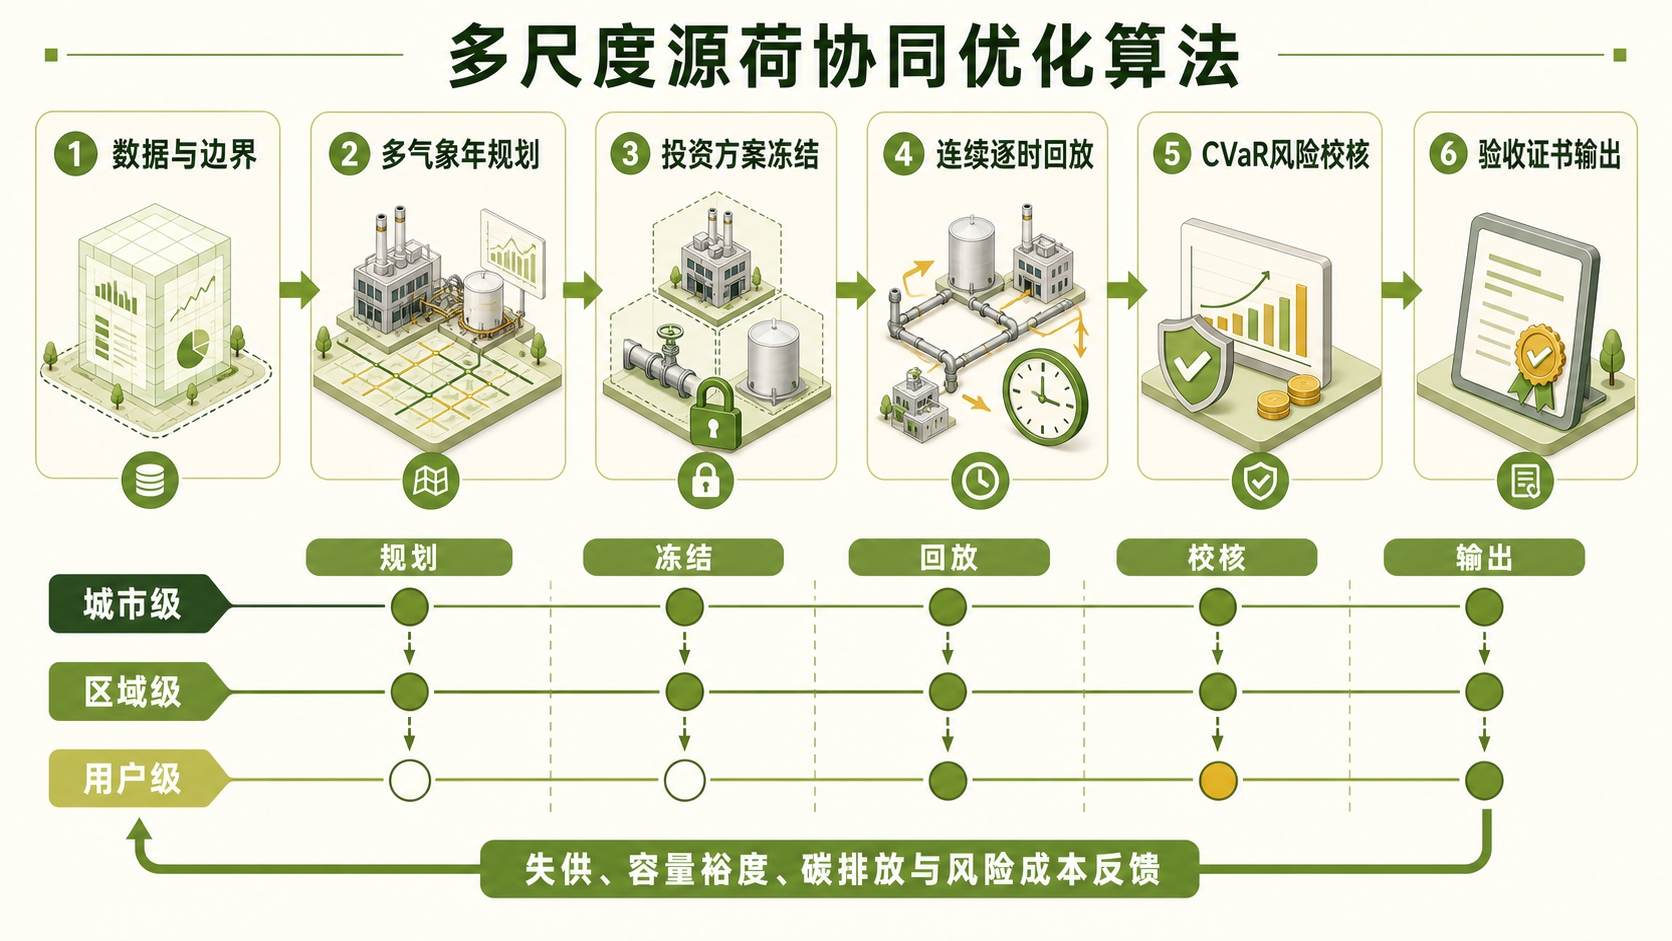
\includegraphics[width=0.76\textwidth,height=0.38\textheight,keepaspectratio]{media/algorithm-revision/fig1.png}
\caption{多尺度源荷协同优化算法总体流程}
\label{fig:alg-overview}
\end{figure}

与确定性单情景规划及工程手册式方案比选相比，本文算法的主要差异见表\ref{tab:alg-comparison}。

\begin{table}[H]
\centering
\caption{常见做法与本文算法的对照}
\label{tab:alg-comparison}
\begin{tabularx}{\textwidth}{p{0.27\textwidth}p{0.35\textwidth}X}
\toprule
常见做法 & 本文算法 & 核验依据\\
\midrule
逐时离散化、确定性单情景规划 & 1~h全季求解，并开展多情景与极端年全年回放 & 主解求解记录、极端年累计61392~h回放\\
采用规划手册指标评价方案 & 单一MILP主解，并进行$\varepsilon$-约束与风险扫描 & 求解状态、上下界和相对间隙\\
规划与运行分开处理 & 三场景同一条管线：代表时段投资---运行联合规划，再冻结投资完成全季运行校核 & 规划层与回放层分别记录状态和间隙\\
\bottomrule
\end{tabularx}
\end{table}

\subsection{多尺度模型}

模型由城市层、区域层和用户层构成，各层通过共享投资变量、逐时运行变量和状态耦合约束连接。三个算例均采用3个聚合负荷节点；乌鲁木齐、固原和武汉分别包含7、6、7类热源和3、2、1条聚合管段。城市层对应总体投资与技术路线，区域层对应热源和输配单元，用户层对应同类建筑负荷的聚合节点。其关系如图\ref{fig:alg-multiscale}所示。

\begin{figure}[H]
\centering
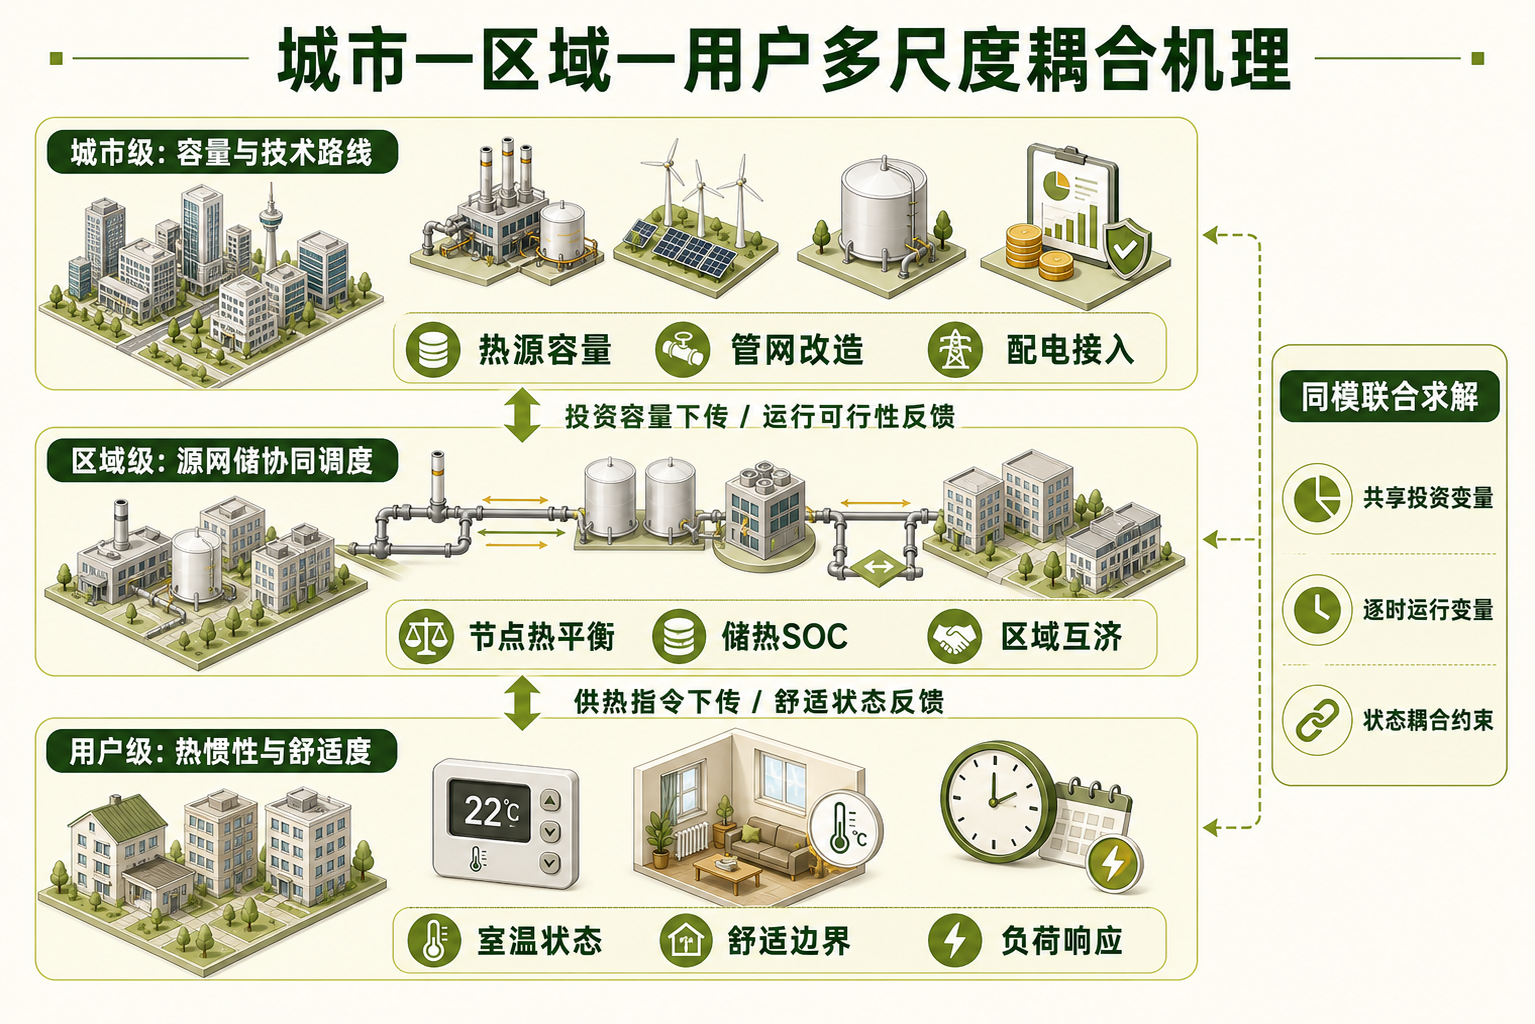
\includegraphics[width=0.76\textwidth,height=0.30\textheight,keepaspectratio]{media/algorithm-revision/fig2.png}
\caption{城市---区域---用户多尺度耦合机制}
\label{fig:alg-multiscale}
\end{figure}

城市层确定容量与技术路线，包括新增或退役机组容量、热源温位模式、候选管径、储热规模以及配电接入和增容。候选技术链依据资源、场地、配电和政策条件生成并预筛，本次计算执行容量、拓扑和温级预审。

区域层描述能流、管网与储热。模型在节点和75/45~$^{\circ}$C两级温位上建立逐时能量平衡。温位兼容约束阻止低温热源直接供应高温需求，高温热源供应低温需求时将品位损失计入火用失配惩罚：
\begin{equation}
T_{\mathrm{src}}^{\min}\geq T_{\mathrm{sup}}+\Delta T_{\mathrm{he}},
\label{eq:alg-grade}
\end{equation}
其中，$T_{\mathrm{src}}^{\min}$为热源供水温度下界，$T_{\mathrm{sup}}$为用户供水温度要求，$\Delta T_{\mathrm{he}}$为换热端差。管网采用温位线性化和双向流动互斥约束，储热状态按下式递推：
\begin{equation}
E_{s,t}=(1-\mu_s)E_{s,t-1}+\eta_{\mathrm{ch}}q_{s,t}^{\mathrm{ch}}\Delta t-\frac{q_{s,t}^{\mathrm{dis}}\Delta t}{\eta_{\mathrm{dis}}},
\label{eq:alg-storage}
\end{equation}
其中，$\mu_s$为自损失率，$\eta_{\mathrm{ch}}$和$\eta_{\mathrm{dis}}$分别为充、放热效率。

用户层描述聚合节点的热惯性与负荷调节。状态上下界、需求响应窗口守恒和参与率上限共同约束用户侧调节行为。凡启用楼栋级室温递推的算例，其室温按一时段内热输入不变条件下的精确离散递推：
\begin{align}
a_n&=\exp\!\left(-H_n\Delta t/C_n\right),\qquad \beta_n=\frac{1-a_n}{H_n},\\
\theta_{n,t}&=a_n\theta_{n,t-1}+(1-a_n)T_t^{\mathrm{out}}
+\beta_n\!\left(Q_{n,t}^{\mathrm h}-Q_{n,t}^{\mathrm c}+G_{n,t}\right),
\label{eq:alg-building}
\end{align}
其中，$\theta_{n,t}$为时段末室温，$C_n$为等效热容，$H_n$为围护与通风合并的总传热系数，$G_{n,t}$为内部与太阳得热之和。该式是时段内输入不变时的精确积分，不是差分近似。本条与式\eqref{eq:load-decomp}后的聚合等效蓄热描述的是两套不同对象：三场景主链采用聚合等效热状态，楼栋级室温用于启用该模块的算例并单独登记初末温度，两者不互相替代，也不共用初末边界。

三个尺度通过容量、温位和建筑改造三类连接相互约束：容量约束将运行出力限制在可用率及设备上下限内；温位匹配表完成“源温---网温---节点负荷”匹配；用户侧调节量先进入节点热平衡，再由热源出力与储热充放共同响应。例如在已有逐时结果中，用户侧负荷削减使同一时段节点需求下降，优先减少边际热源出力；恢复负荷出现时，储热先放热并由可调热源补足剩余需求，节点平衡在每个时段保持闭合。三个场景采用同一条求解管线：先在代表时段上完成投资---运行联合规划，再冻结投资方案进行完整时序运行校核；规划层与回放层分别报告求解状态与相对间隙。因此，推荐方案用于工程可行性比较，不将代表时段投资层的结果表述为全季最优。

\subsection{多目标协同优化}

成本与碳排放采用$\varepsilon$-约束法协调，而不直接将不同量纲的成本和碳排放加权相加。模型以全生命周期净成本的等年值最小为目标，同时设置碳排放上限；逐档收紧上限并重新求解完整供暖季，相邻两档的成本增量与减排量之比用于计算边际减排成本。

乌鲁木齐场景中，成本端点为27.49万元、27.32~t~CO$_2$，排放端点为74.81万元、10.57~t~CO$_2$。本文推荐记录采用通过全部硬约束与工程检查的方案，等年值成本为27.76万元、碳排放为27.31~t~CO$_2$；该记录与仅按目标函数排序得到的成本端点分开标注。单位供热成本由基准方案的0.078851元/kWh增至0.100681元/kWh，增加27.69\%。该增幅反映以成本增加换取减排、清洁热利用和可靠性约束的综合取舍。

零失供、清洁热比例、N$-1$容量裕度、地源年度平衡和舒适度上下限作为硬边界，不与经济性目标交换。失供率约束为
\begin{equation}
U_{\mathrm{un}}=\frac{\sum_t q_t^{\mathrm{un}}}{\sum_t Q_t}\leq U_{\max},
\label{eq:alg-unserved}
\end{equation}
其中，$q_t^{\mathrm{un}}$为失供功率，$Q_t$为热需求，$U_{\max}=0$表示推荐方案不允许失供。边界内的需求移峰和舒适偏差通过惩罚成本进行优化。

气象不确定性作为独立风险层，采用
\begin{equation}
\min\ \mathbb{E}[C]+\lambda\operatorname{CVaR}_{\alpha}(C),
\qquad \alpha=0.8,
\label{eq:alg-risk-objective}
\end{equation}
其中，$\lambda$取0、0.02、0.05和0.10四档。条件风险价值采用Rockafellar--Uryasev线性化：
\begin{equation}
\operatorname{CVaR}_{\alpha}(C)=\min_{\eta,z_s}\left\{\eta+\frac{1}{1-\alpha}\sum_s p_sz_s\right\},
\quad z_s\geq C_s-\eta,\quad z_s\geq0.
\label{eq:alg-cvar}
\end{equation}

$\lambda=0.05$作为三个场景的统一参考值。多气象年风险层中，乌鲁木齐的期望成本增加0.012万元、CVaR下降0.831万元；固原的期望成本增加0.016万元、CVaR下降0.515万元，变化约占年化成本的0.01\%。武汉场景的投资不随风险权重改变，说明其投资方案主要由硬约束决定。不同风险权重下的结构变化见表\ref{tab:alg-lambda}。

\begin{table}[H]
\centering
\caption{多气象年风险层的$\lambda$权重扫描结果}
\label{tab:alg-lambda}
\begin{tabularx}{\textwidth}{cXXX}
\toprule
$\lambda$ & 乌鲁木齐 & 固原 & 武汉\\
\midrule
0.02 & 余热源热泵、备用电锅炉和配电容量首次调整 & 投资配置不变 & 投资配置不变\\
0.05 & 继续小幅调整 & 储热与微网可再生增加，生物质调峰减少 & 投资配置不变\\
0.10 & 进一步转入风险平衡 & 与0.05档接近 & 投资配置不变\\
\bottomrule
\end{tabularx}
\end{table}

$\lambda$扫描来自2020---2024多气象年全年回放，用于风险机制专项验证；供暖季主结果中的成本---碳Pareto采用确定性单情景计算。风险层共包含12个规划案例（3个场景$\times$4档$\lambda$），全部收敛，60项年度容量审计通过，CVaR一致性核验误差为$5.59\times10^{-9}$元。图\ref{fig:alg-objectives}展示的是该专项风险层的12/12案例收敛与60/60容量审计结果，不等同于供暖季推荐方案的13道机器验收。

\begin{figure}[H]
\centering
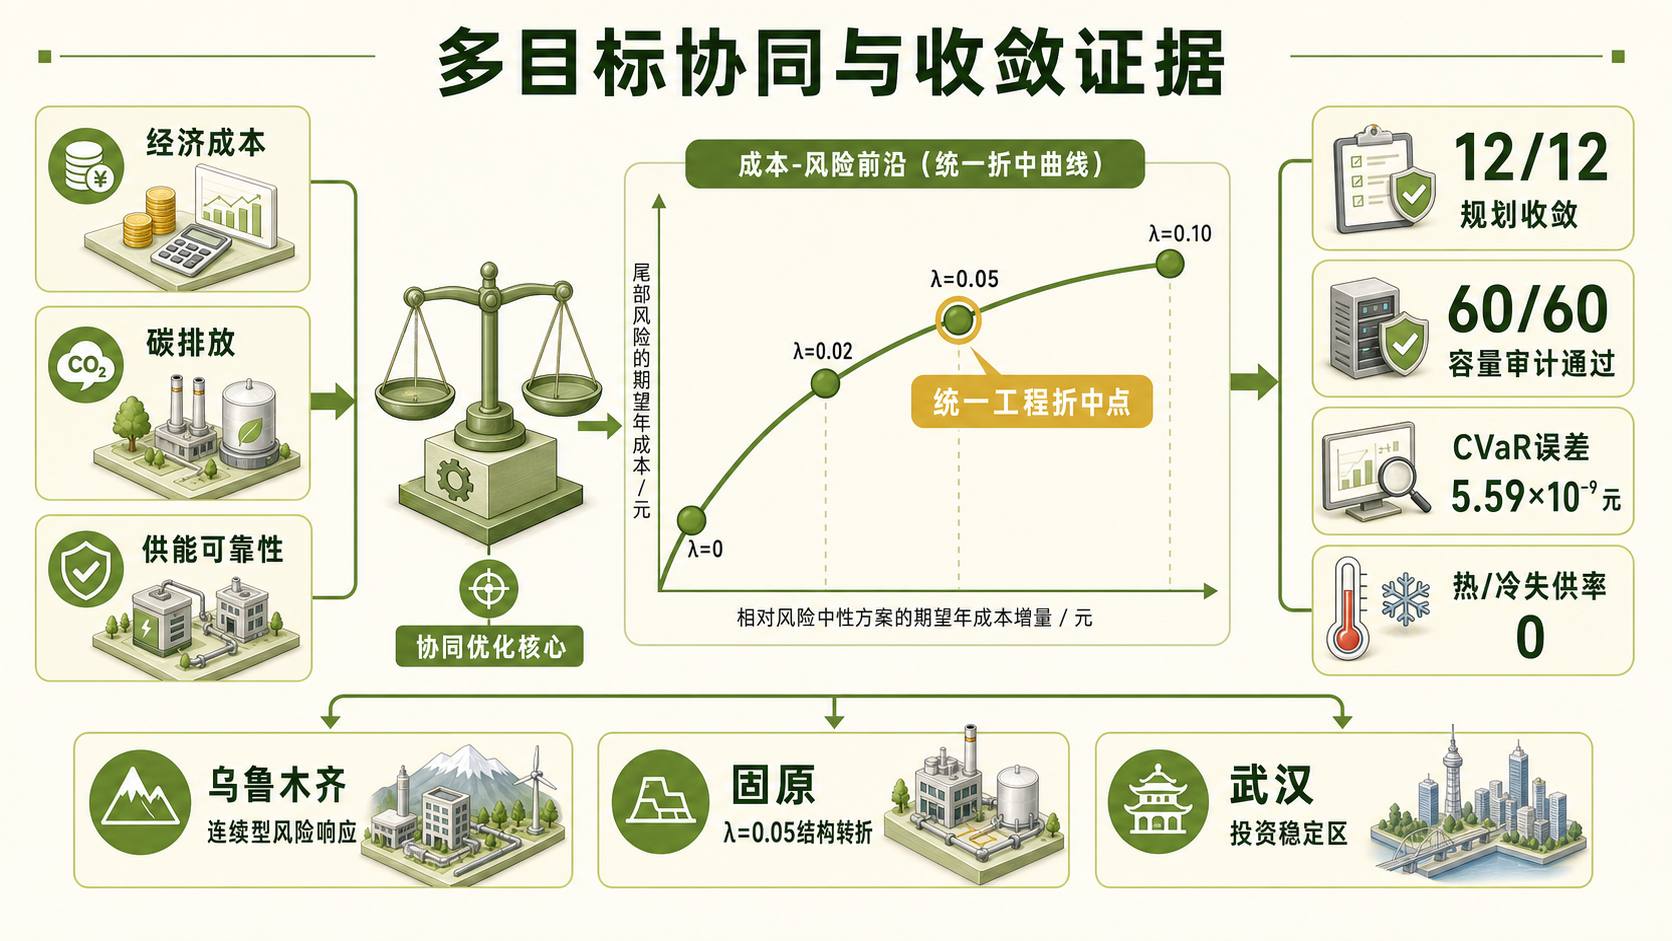
\includegraphics[width=0.76\textwidth,height=0.30\textheight,keepaspectratio]{media/algorithm-revision/fig3.png}
\caption{多目标协同与风险层收敛证据}
\label{fig:alg-objectives}
\end{figure}

\subsection{求解流程与收敛准则}

模型构造器采用Python~3.11实现，并通过SciPy的\texttt{milp}接口调用HiGHS求解。约束矩阵按CSR/CSC稀疏格式编译和缓存，模型装配约需1.6~s，未使用自定义割。机组启停采用凸包重建模，开机状态保留为二元变量，启动和停机辅助变量连续化。全年回放单城测试中，整数变量数量由26280个减至8760个。

求解流程包括四步：首先完成配置与指标初始化；其次进行候选技术链预筛；然后按$\varepsilon$-约束或风险权重批量求解；最后进行逐时回放和验收审计。收敛需同时满足以下条件：求解状态达到全局最优或允许间隙并具有上下界证明；可行解与对偶界形成可解释的相对MIP gap；约束残差不超过$10^{-6}$；逐时回放与后验复核通过。

表\ref{tab:alg-solver}登记三个场景代表时段规划阶段的求解记录。该组数值为初赛轮次的实验记录：代表时段规划层相对间隙分别为$1.53\times10^{-4}$、$1.84\times10^{-3}$和0.98\%，逐时热平衡最大绝对残差依次为$7.41\times10^{-13}$、$1.25\times10^{-10}$和$8.53\times10^{-14}$~kW。该组记录未随附可回查的求解日志，本稿以历史报告值列出，逐行核验状态见表中「来源状态」列；本次补充验证可回查的同类记录见表\ref{tab:alg-supplement}。

\begin{table}[H]
\centering
\caption{三场景代表时段规划求解记录（历史报告值）}
\label{tab:alg-solver}
\small
\begin{tabularx}{\textwidth}{@{}p{0.07\textwidth}p{0.13\textwidth}p{0.12\textwidth}p{0.08\textwidth}p{0.12\textwidth}p{0.17\textwidth}X@{}}
\toprule
场景 & 求解方法 & 整数变量 & 时间/s & 相对间隙 & 来源状态 & 验收\\
\midrule
乌鲁木齐 & 代表时段投资---运行联合规划 & 启停二元8784个 & 531.1 & $1.53\times10^{-4}$ & 初赛记录，无日志 & 原稿记载通过（未核验）\\
固原 & 代表时段投资---运行联合规划 & 启停二元4392个 & 64.0 & $1.84\times10^{-3}$ & 初赛记录，无日志 & 原稿记载通过（未核验）\\
武汉 & 代表时段投资---运行联合规划 & 0 & 31.7 & 0.98\% & 初赛记录，无日志 & 原稿记载通过（未核验）\\
\bottomrule
\end{tabularx}
\end{table}

表\ref{tab:alg-supplement}为本次修订实际执行并留存的补充验证。三个场景在同一套来源锁定的公开输入上，按“代表时段规划---冻结投资---可靠容量审计---全年连续回放”顺序求解；求解状态、可行目标值、求解下界、相对间隙、耗时、逐时残差与违约小时均取自落盘的运行记录。

\begin{table}[H]
\centering
\caption{补充验证：三场景冻结投资全年回放求解与验收登记}
\label{tab:alg-supplement}
\small
\begin{tabularx}{\textwidth}{@{}p{0.07\textwidth}p{0.05\textwidth}p{0.055\textwidth}p{0.135\textwidth}p{0.085\textwidth}p{0.115\textwidth}p{0.085\textwidth}p{0.055\textwidth}X@{}}
\toprule
场景 & 阶段 & 终止状态 & 可行值 / 下界（万元） & 相对间隙 & 最大约束违反量 & 耗时/s & 失供率 & 验收项\\
\midrule
乌鲁木齐 & 规划 & 0 & 65.788 / 65.661 & $1.93\times10^{-3}$ & $5.190\times10^{-11}$ & 0.94 & 0 & ---\\
乌鲁木齐 & 回放 & 0 & 66.065 / 66.012 & $8.13\times10^{-4}$ & $9.963\times10^{-7}$ & 49.46 & 0 & 15/15\\
固原 & 规划 & 0 & 135.774 / 135.770 & $3.17\times10^{-5}$ & $6.253\times10^{-13}$ & 14.87 & 0 & ---\\
固原 & 回放 & 0 & 138.057 / 137.410 & $4.69\times10^{-3}$ & $9.997\times10^{-7}$ & 32.60 & 0 & 16/16\\
武汉 & 规划 & 0 & 54.603 / 54.603 & 0 & $8.188\times10^{-13}$ & 0.80 & 0 & ---\\
武汉 & 回放 & 0 & 56.029 / 56.029 & 0 & $8.837\times10^{-7}$ & 74.28 & 0 & 17/17\\
\bottomrule
\end{tabularx}
\end{table}

\noindent{\footnotesize 注：「终止状态」列为求解器返回状态，0 表示按登记的绝对容差 $10^{-6}$、相对容差 $10^{-8}$ 与相对间隙阈值判定最优；相对间隙非零的行，其最优性在该登记容差内成立。「最大约束违反量」取该阶段数值审计的最大约束违反量，单位为对应约束自身的单位。储热状态方程最大残差与各储热装置的初末状态另见同包交付的《仿真结果数据表》。}

该组回放覆盖2023年完整日历年8760~h，时间步长1~h，验证同一模型与配置在完整年时间轴上的连续性与可靠性；主结果供暖季窗口的登记与核验状态见表\ref{tab:alg-solver}的「来源状态」列。武汉的两阶段求解在补齐代表时段锚点后通过全部验收项；未补齐时其冻结投资方案因并网可靠电力容量低于全年需求$0.1058$~kW而被就绪审计拒绝，该锚点修正与新旧容量对照登记于同包交付的《仿真结果数据表》。

敏感性测试的20档扰动获得有效解，其中乌鲁木齐电价高档和余热低档为时间受限近似解，相对间隙分别为7.05\%和9.44\%；另有固原负荷低档、武汉碳价高档两档未收敛。乌鲁木齐Pareto中间档的部分点在时限内间隙为13.2\%---13.7\%。固原三档采用推荐投资模式复算，全部满足碳排放上限，间隙为0.20\%、0.22\%和0.24\%，这些结果属于冻结投资模式的运行参考点，不代表完整联合MILP重新寻优。

为检验乌鲁木齐排放端点投资模式在不同碳帽下的运行可达性，固定排放最优解的投资、退役、管径、储热和末端改造模式，对23365、19136和14906~kg三档碳帽进行全季运行重算。三档实际排放均为10616.5~kg，失供率为0，求解状态均为Optimal，相对间隙为$1.90\times10^{-7}$。运行成本为11.271万元/年，仅包含运行费用，不与联合解中包含资本成本的Pareto结果直接比较。

\subsection{计算效率与扩展性}

求解效率的改善主要来自启停凸包重建模和稀疏编译缓存。固原全年回放用时由575.746~s降至86.903~s，提升6.63倍；两年度合计用时由602.483~s降至112.750~s，减少81.29\%。该结果来自多气象年全年回放的单城效率测试。单次供暖季问题约包含31万---45万个变量，乌鲁木齐场景的启停二元变量为8784个。连续温位、C\&CG、Benders分解和在线MPC作为可选扩展，本次计算未启用。逐时回放、边界检验和求解加速关系如图\ref{fig:alg-replay}所示。

\begin{figure}[H]
\centering
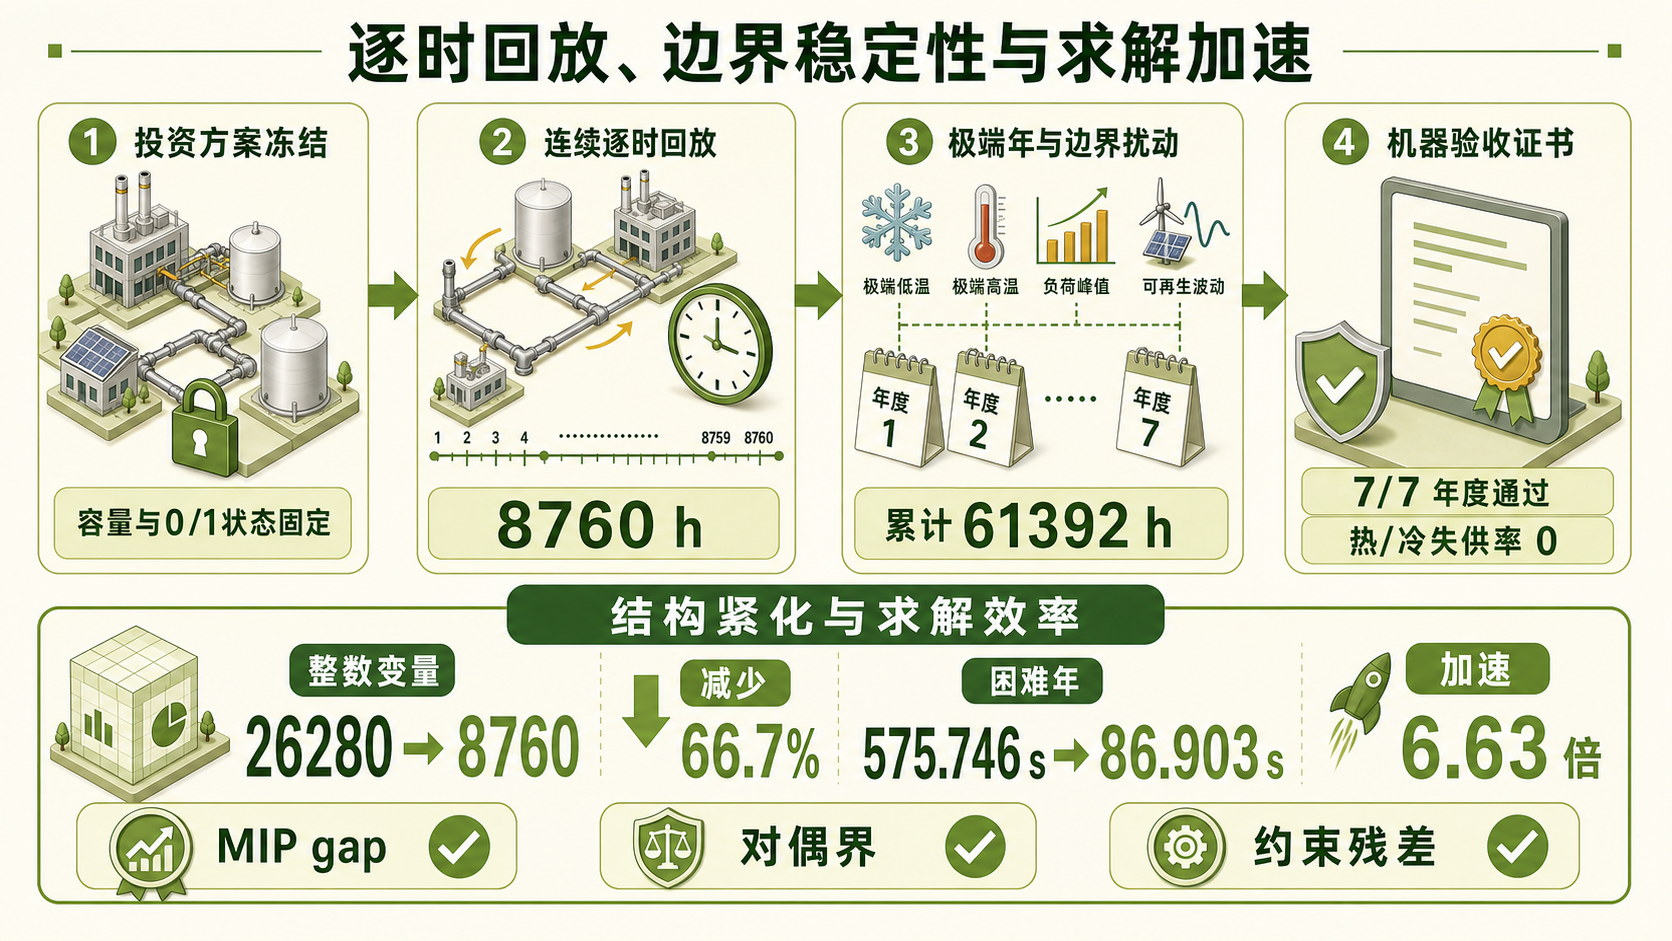
\includegraphics[width=0.76\textwidth,height=0.30\textheight,keepaspectratio]{media/algorithm-revision/fig4.png}
\caption{逐时回放、边界稳定性与求解效率}
\label{fig:alg-replay}
\end{figure}

\subsection{数值结果与敏感性}

图\ref{fig:code-kpi}比较了基准方案与推荐方案的成本、碳排放、清洁热利用和供热可靠性指标。推荐方案的取舍由成本、排放上限、清洁热占比和供热约束共同决定，因此各项指标的变化方向并不完全一致。图中成本采用年化等效值，单位供热成本按交付热量折算，二者与供暖季现金运行成本分别核算。

\begin{figure}[H]
\centering
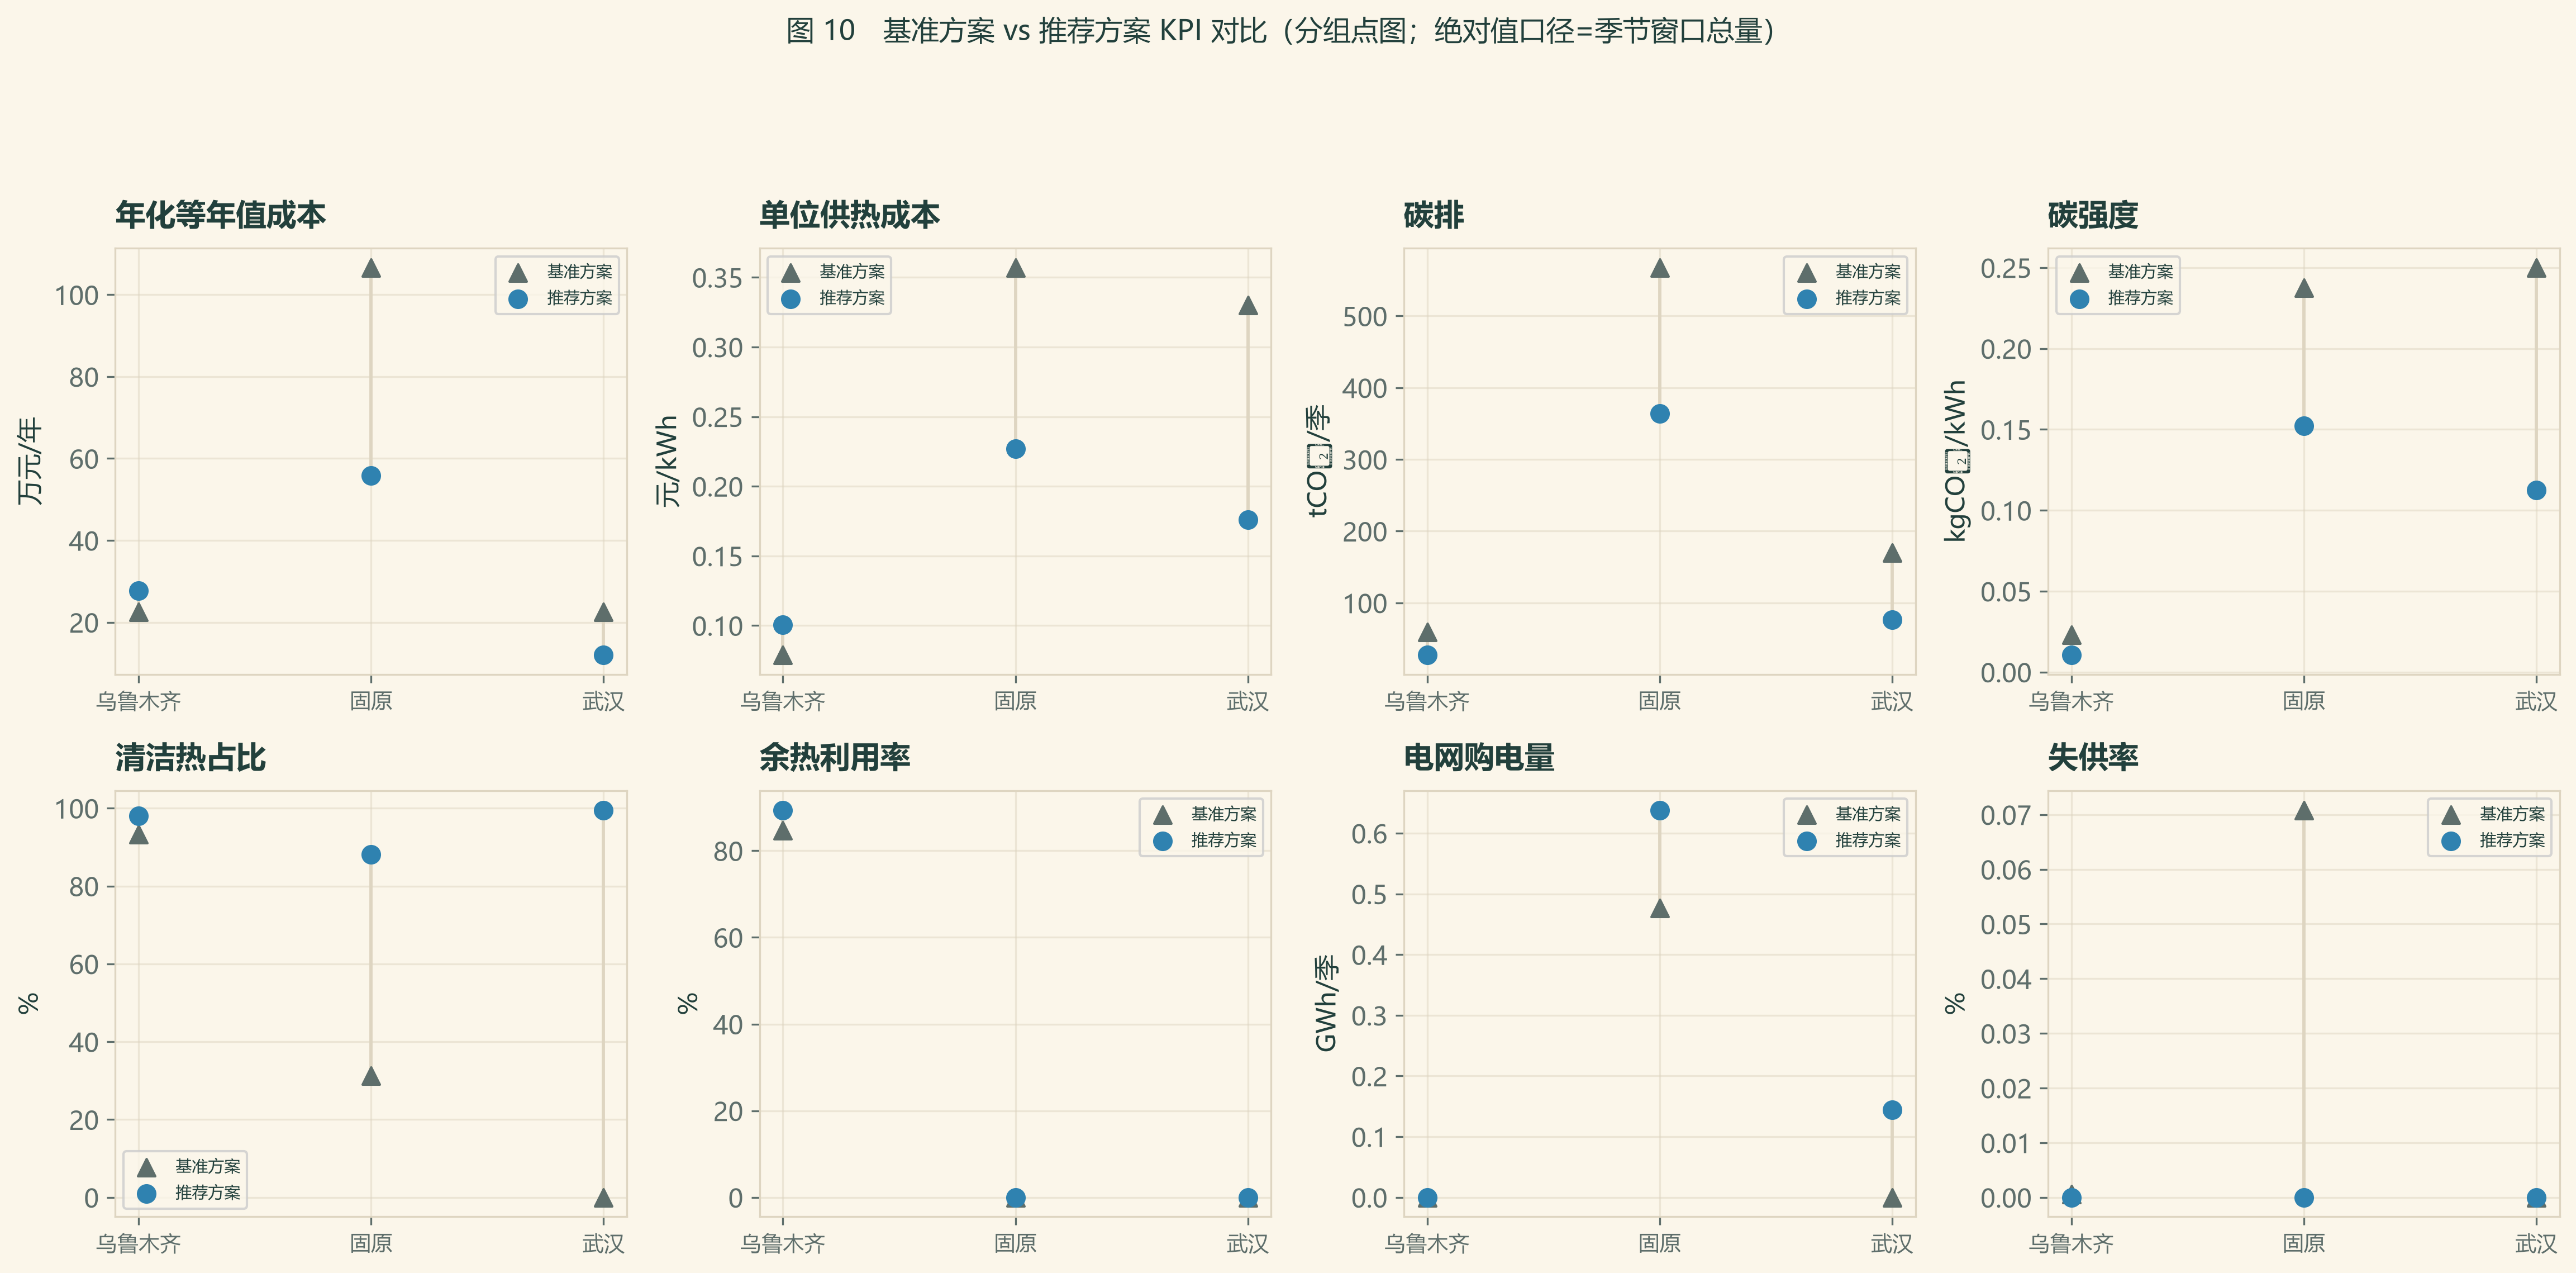
\includegraphics[width=0.98\textwidth,height=0.52\textheight,keepaspectratio,trim=0 0 0 100,clip]{media/code-results/fig10_kpi_comparison.png}
\caption{基准方案与推荐方案KPI对比}
\label{fig:code-kpi}
\end{figure}

成本与碳排放的候选解分布见图\ref{fig:code-pareto}。推荐方案从满足排放、可靠性和投资边界的候选解中选取，不必与最低成本点或最低排放点重合。部分点为固定投资模式下的运行参考点或时限内近似解，其求解状态和相对间隙以前文说明为准。

\begin{figure}[H]
\centering
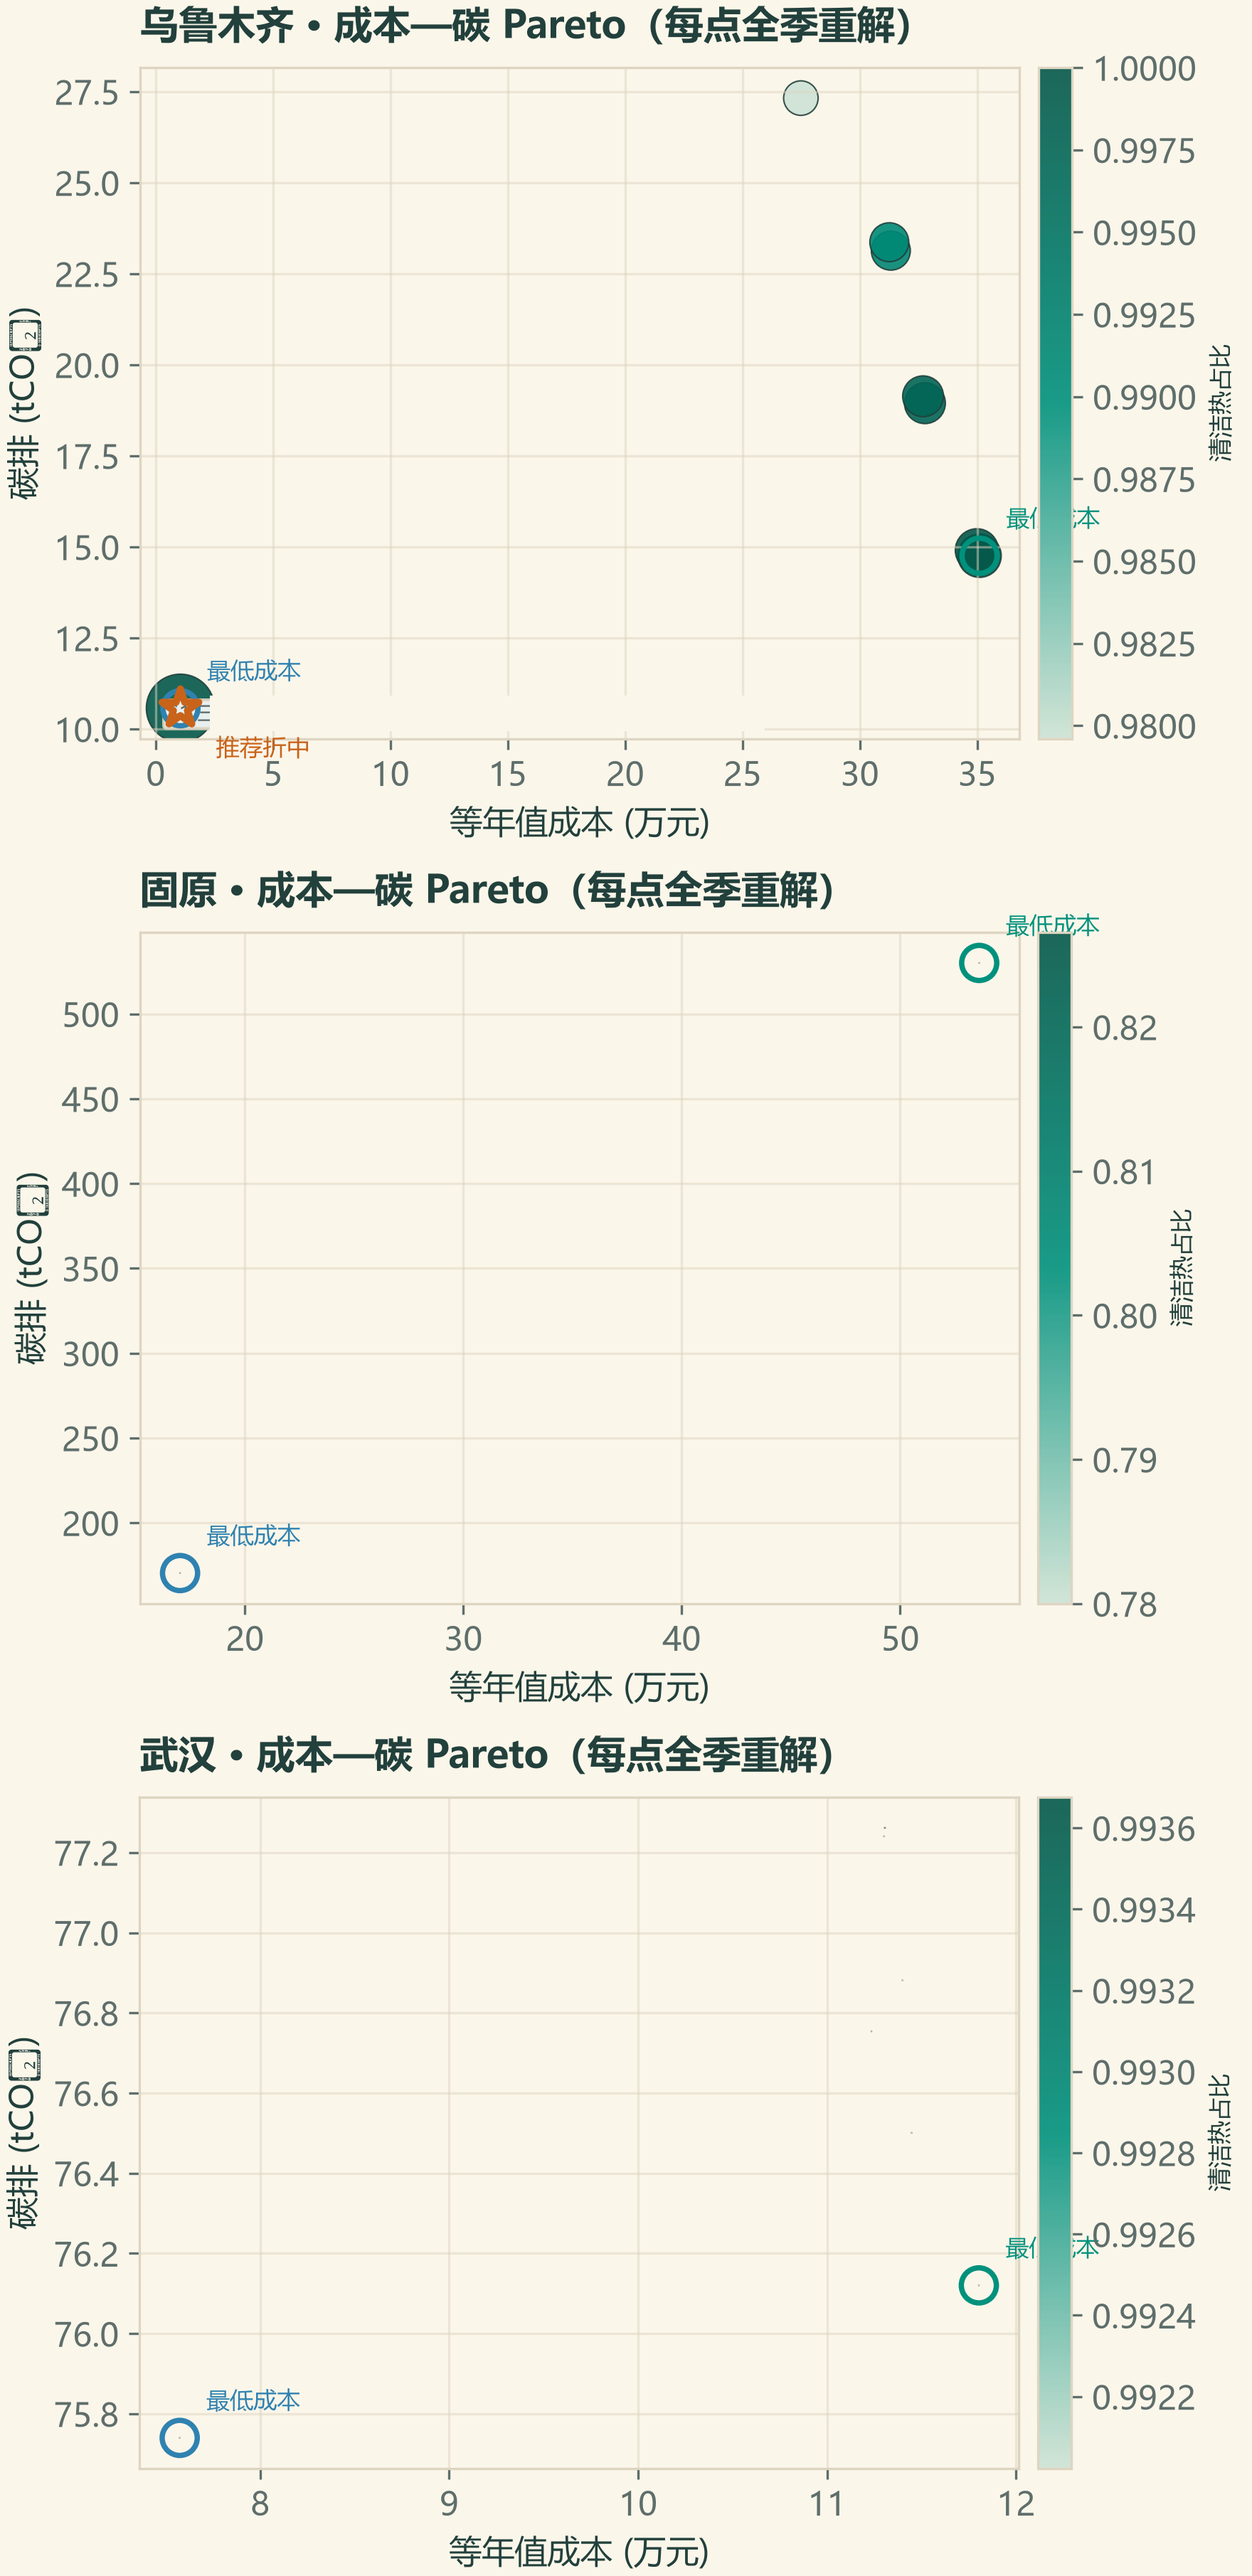
\includegraphics[width=0.82\textwidth,height=0.82\textheight,keepaspectratio]{media/code-results/fig11_cost_emission_pareto_stack.png}
\caption{三城市成本—碳排放候选方案对比（气泡大小为年化新增投资；乌鲁木齐面板左下重叠的三个标记分别为最低成本、推荐折中与同一位置上的时限内可行解，其中时限可行解的相对间隙为 13.2\%---13.7\%，最优性未证明）}
\label{fig:code-pareto}
\end{figure}

V4全年单情景消融实验沿用原时间权重，并在每次移除模块后重新求解投资与运行。完整模型的年化目标为95.620万元，碳排放为30.602万kg~CO$_2$。去掉需求响应后，年化成本增加0.09\%，购电量增加0.21\%；去掉新增储热后，年化成本增加3.55\%，碳排放增加6.05\%，购电量增加3.41\%；去掉火用失配惩罚后，火用损失增加4.90\%。该组结果用于检验V4模块贡献，与三城市供暖季推荐方案分开报告。

复合寒潮压力测试沿用V4算例，将室外温度序列整体降低8~$^{\circ}$C、负荷提高15\%、余热可用量降低15\%，并冻结投资变量。测试结果仍保持零失供；既有实验记录报告\textbf{运行目标值}增加18.55\%，购电量增加56.78\%，碳排放增加113.95\%。运行目标值含年化投资、碳成本、启停、运维与惩罚项，与能源现金支出分别核算，两者不可互相换算；该记录未随附可回查日志。逐档敏感性分析表明：乌鲁木齐对热负荷最敏感，成本变化为$+19.1\%/-17.9\%$，其次为余热下降和电价上升；固原的生物质到货扰动因库存缓冲未改变成本；武汉对电价和热负荷较敏感，变化范围分别为$+16.9\%/-14.6\%$和$+16.8\%/-13.7\%$。

最冷连续168~h的热源出力、负荷和储热状态见图\ref{fig:code-cold168}，用于检查低温持续期间的逐时供需平衡。图\ref{fig:code-worst72}进一步列出最不利72~h窗口内的可用供热能力、负荷、储热与容量裕度。两图分别反映常规极寒时段调度和压力场景下的边界状态，不据此假定三城市具有相同的储热运行模式。

\begin{figure}[H]
\centering
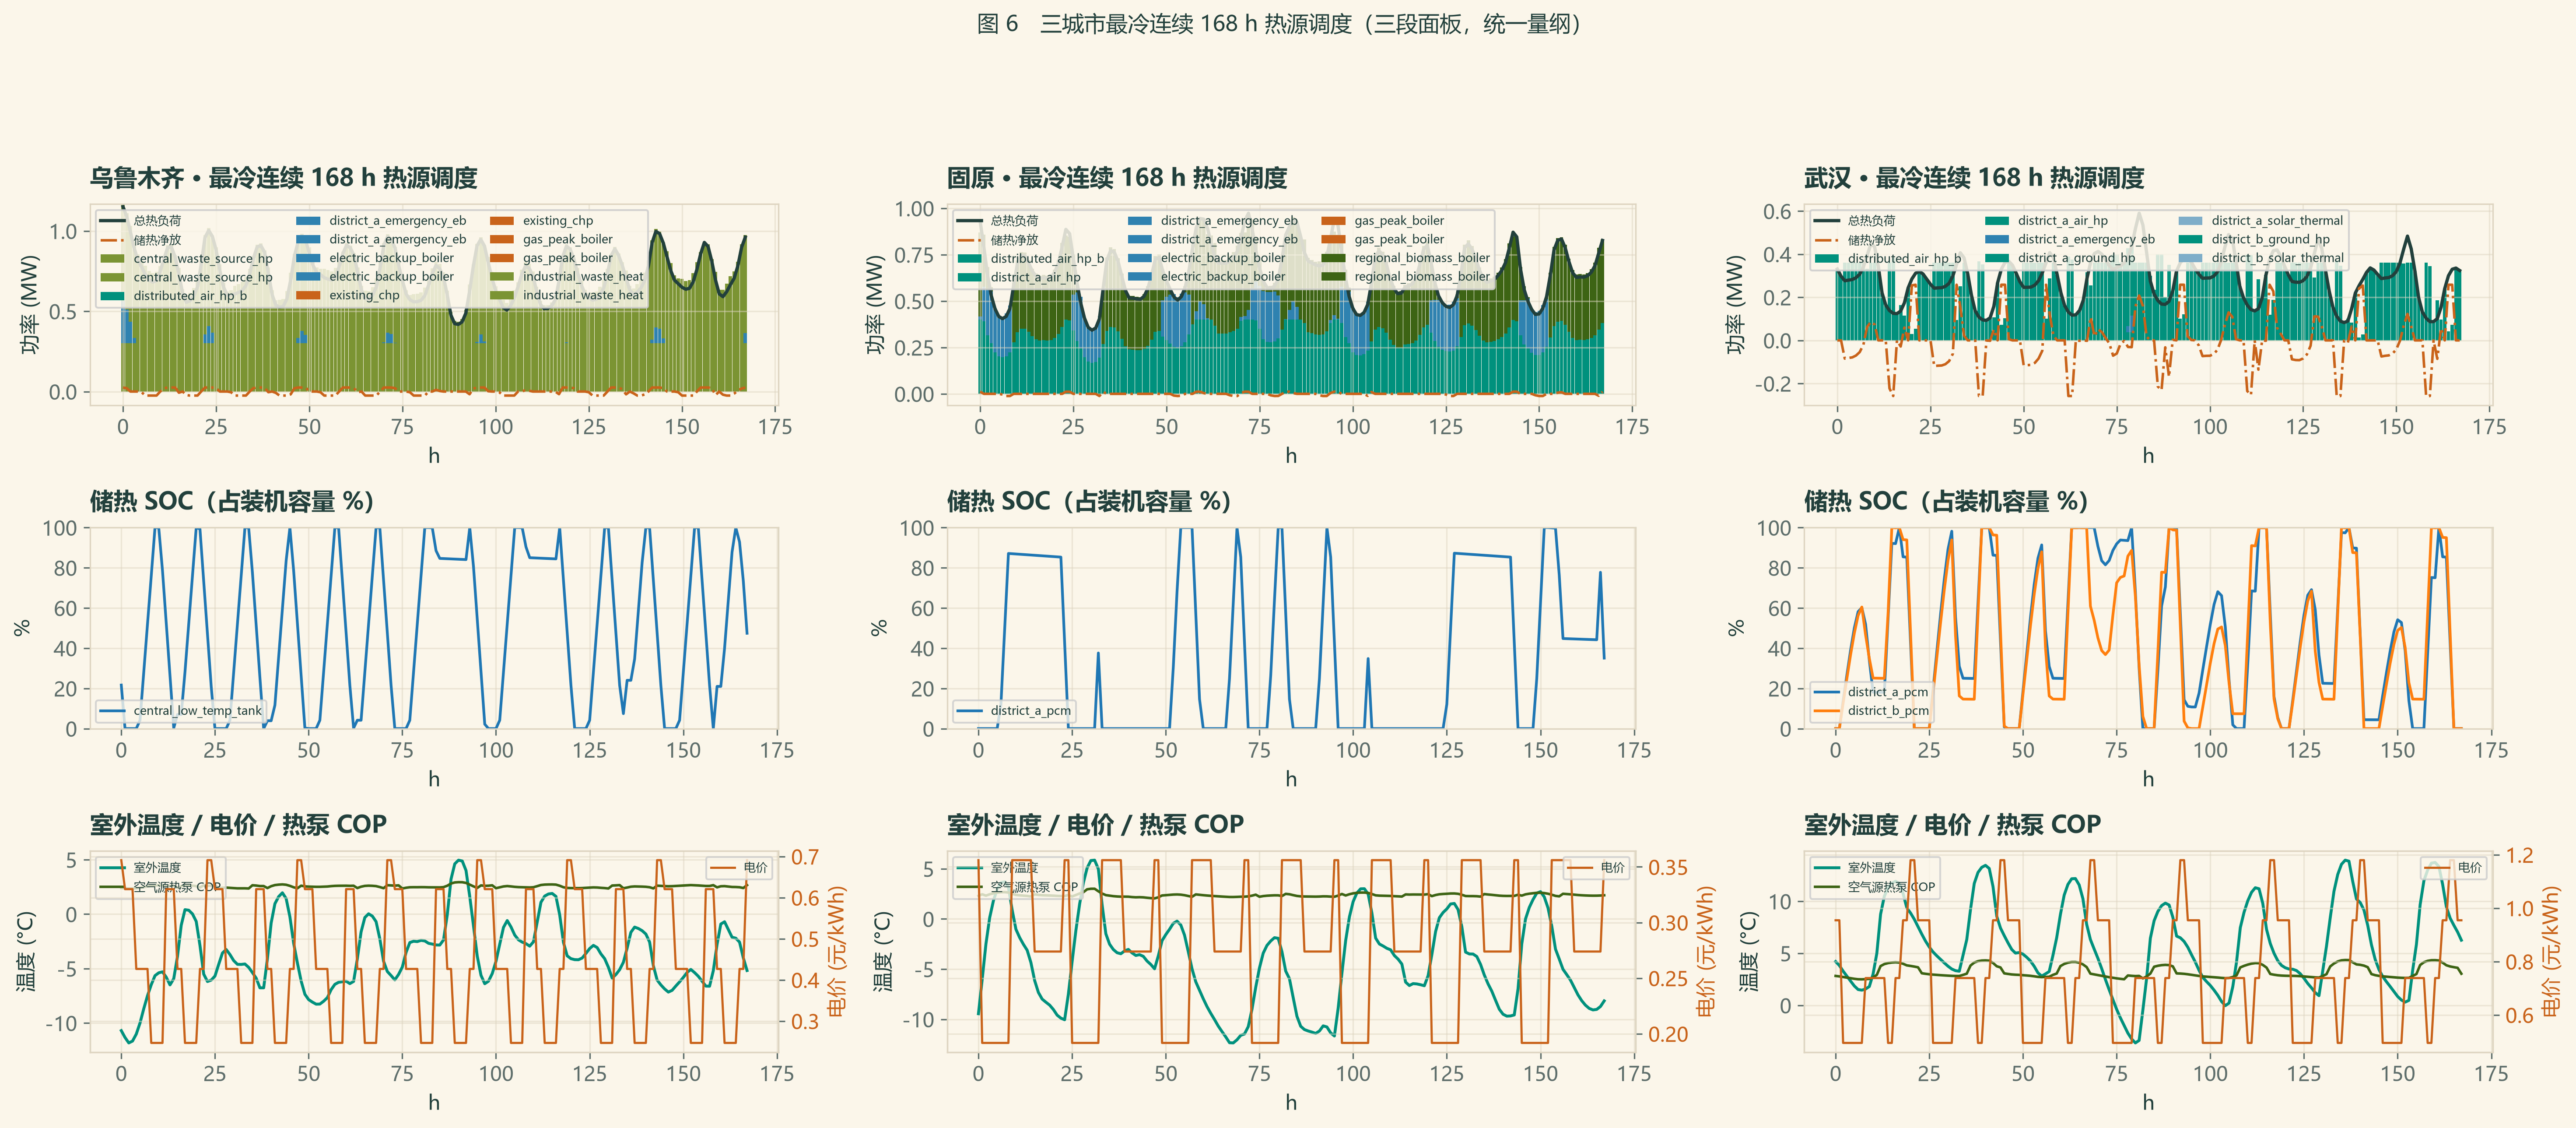
\includegraphics[width=0.98\textwidth,height=0.54\textheight,keepaspectratio,trim=0 0 0 100,clip]{media/code-results/fig06_coldest_168h_dispatch.png}
\caption{最冷连续168 h调度}
\label{fig:code-cold168}
\end{figure}

\begin{figure}[H]
\centering
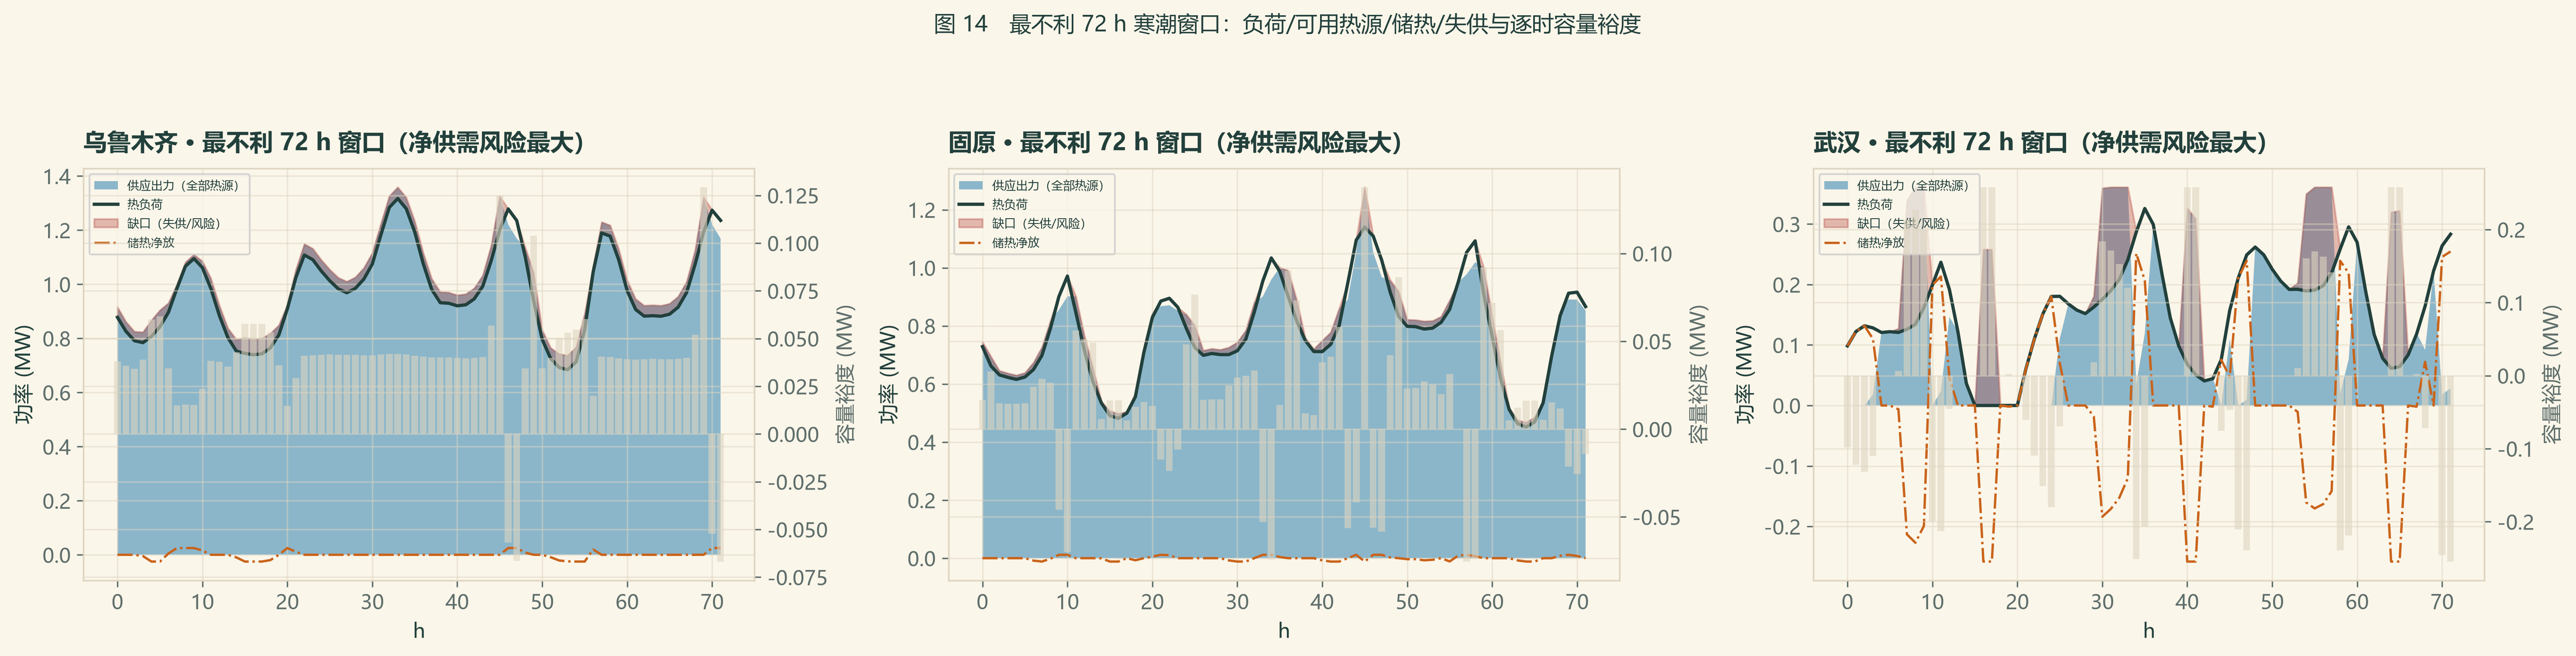
\includegraphics[width=0.98\textwidth,height=0.43\textheight,keepaspectratio,trim=0 0 0 100,clip]{media/code-results/fig14_worst_72h_resilience.png}
\caption{最不利72 h韧性窗口}
\label{fig:code-worst72}
\end{figure}

与“单年或五年聚合代表时段、最小化平均成本”的基准相比，多气象年回放使用约3---4倍代表行数，5个气象年的容量审计均通过，最差场景失供率仍为0。消融实验、压力测试和数据可靠性分级见图\ref{fig:alg-ablation}。

\begin{figure}[H]
\centering
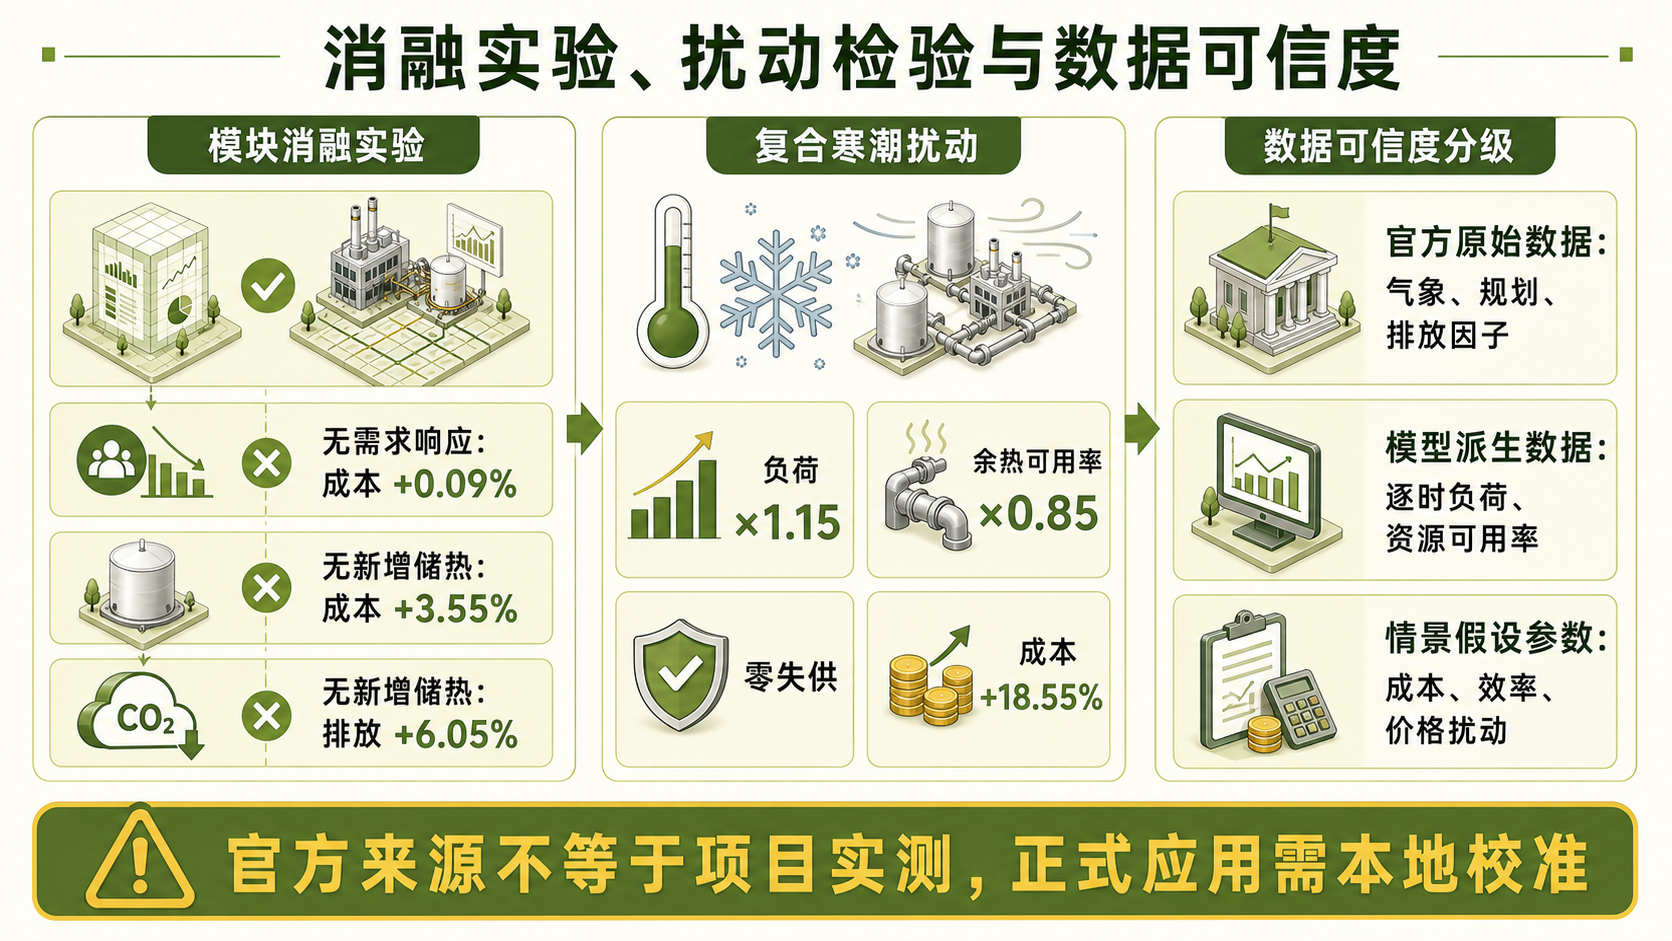
\includegraphics[width=0.76\textwidth,height=0.30\textheight,keepaspectratio]{media/algorithm-revision/fig5.png}
\caption{消融实验、扰动检验与数据可靠性}
\label{fig:alg-ablation}
\end{figure}

\subsection{数据基础与适用范围}

气象数据采用NASA POWER格点逐时数据，空间分辨率为$0.5^{\circ}\times0.625^{\circ}$，不作为地面站实测数据。热工参数、项目容量和政策边界取自标准、批复与政府文件；设备成本、燃料价格等作为情景假设并给出区间。数据记录包括来源、链接、检索时间、单位、分辨率、换算公式和适用局限。

碳排放按逐时电力排放因子计算，由输入时序列\texttt{grid\_emission\_factor}逐时读取，不作常数处理。本次补充验证三场景回放所用该列的取值个数为 17---19 个，范围为 $0.43$---$0.69$~kg~CO$_2$/kWh，全年均值约 $0.535$---$0.546$。作为参考，2023 年全国电力平均排放因子为 0.5306~kg~CO$_2$/kWh，新疆、宁夏和湖北的省级年度参考因子分别为 0.6021、0.6187 和 0.4044~kg~CO$_2$/kWh。同包交付的《仿真结果数据表》中，共享容量原型对照单独采用湖北省年度因子 0.4044，与主场景的逐时因子分属不同登记值；改用统一常数因子重算属于后续可补充的对照工作。三场景均为代表性多节点系统，缩比系数仅用于规模换算，不表示对城市地理系统的完整复刻，横向比较采用单位指标。

\subsection{小结}

算法采用$\varepsilon$-约束处理成本与碳排放的多目标关系，以硬边界约束可靠性，并以$\lambda$-CVaR描述风险态度。三个场景采用同一条“代表时段投资---运行联合规划，再冻结投资完成全季运行校核”的管线，规划层与回放层分别报告求解状态与间隙。多尺度耦合通过节点---温位聚合、用户侧等效热状态以及城市、区域与用户层之间的共享变量实现。

本次补充验证的对应记录见表\ref{tab:alg-supplement}与同包交付的《仿真结果数据表》，其中三个场景的冻结投资全年回放均取得已证最优或容差内最优解，失供率为 0。前述历史报告值的逐行核验状态见相应表格的「来源状态」列。

当前主要成果为成本---碳排放二维$\varepsilon$-约束扫描得到的候选方案集：按有限档位逐档重解，每档报告可行值与对偶界，其中乌鲁木齐中间档的部分点属时限内近似解。该集合是有限档位上的候选解，不等同于对连续前沿的完整刻画。后续可进一步开展三维Pareto扩展、省级排放因子重算，以及连续温位、C\&CG、Benders分解和在线MPC等方法的计算研究。
